\documentclass[conference]{IEEEtran}
\IEEEoverridecommandlockouts

\usepackage{cite}
\usepackage{amsmath,amssymb,amsfonts}
\usepackage{algorithm}
\usepackage{algorithmic}
\usepackage{graphicx}
\usepackage{textcomp}
\usepackage{xcolor}
\usepackage{booktabs}
\usepackage{tabularx}
\usepackage{url}
\usepackage{tikz}
\usetikzlibrary{shapes.geometric, arrows.meta, positioning, calc}

\def\BibTeX{{\rm B\kern-.05em{\sc i\kern-.025em b}\kern-.08em
    T\kern-.1667em\lower.7ex\hbox{E}\kern-.125emX}}

\begin{document}

\title{An Autonomous Media Streaming Architecture with Multi-Provider AI Orchestration, Cascading Subtitle Synthesis, Audio-Visual Boundary Detection, and Behavioral Recommendation Caching}

\author{\IEEEauthorblockN{Manav Sharma}
\IEEEauthorblockA{\textit{Department of Electronics and Communication Engineering} \\
\textit{Maulana Azad National Institute of Technology (MANIT), Bhopal, India} \\
\textit{Platform Engineering \& Distributed Systems Group} \\
Repository: \url{https://github.com/manavsharma111/anime-streaming-website}}
}

\maketitle

\begin{abstract}
Modern over-the-top (OTT) media streaming platforms encounter critical bottlenecks regarding compute-intensive video encoding costs, metadata fragmentation, multi-language accessibility barriers, and user retention. Conventional approaches rely on monolithic transcoder clusters, proprietary third-party captioning services, and crowd-sourced playback markers, which introduce substantial recurring operational costs and single-point-of-failure vulnerabilities. 

This paper proposes an autonomous, cloud-native prototype media streaming architecture designed for distributed video ingestion, resilient multi-provider artificial intelligence (AI) orchestration, and high-throughput content personalization. The architecture integrates: (1) an event-driven, single-decode multi-variant HTTP Live Streaming (HLS) transcoding engine decoupled via BullMQ and Cloudflare R2 zero-egress object storage; (2) a resilient 3-Tier Cascading AI Subtitle Engine combining ultra-low-latency Groq LPUs (\texttt{whisper-large-v3}), OpenAI (\texttt{whisper-1}), and Google Gemini Multimodal Audio (\texttt{gemini-1.5-flash}) for autonomous WebVTT generation; (3) an Autonomous Audio-Visual Opening/Ending (OP/ED) Boundary Detector utilizing heuristic transition filters to identify standard 90-second media segments without external API dependency; and (4) an Implicit Feedback Recommendation Engine driven by watch-completion ratios, reciprocal temporal decay, and Redis in-memory caching.

In an empirical benchmark evaluation across $N = 30$ consecutive paired trials under trans-continental WAN conditions, in-memory caching demonstrated an average latency reduction of 46.5\% (from 1169.16~ms down to 625.99~ms, with median $P_{50}$ falling 48.6\% from 1107.57~ms to 569.08~ms), corroborating a separate preliminary 5-iteration baseline trial (which demonstrated a 44.7\% reduction from 858.84~ms to 475.27~ms). Isolated in-memory cache lookup latency was clocked independently at under 2.5~ms. The architecture establishes a cost-effective, fault-tolerant blueprint for decentralized next-generation streaming systems.
\end{abstract}

\begin{IEEEkeywords}
HTTP Live Streaming (HLS), Adaptive Bitrate (ABR), Speech-to-Text Cascade, Whisper AI, Audio-Visual Transition Filtering, Reciprocal Temporal Decay, Distributed Queues, Cloudflare R2, Redis In-Memory Caching.
\end{IEEEkeywords}

\section{Introduction}
The global demand for high-definition, interactive multimedia streaming has escalated exponentially over the past decade. Video streaming architectures are inherently complex, requiring synchronized coordination across ingestion, multi-bitrate encoding, global content delivery networks (CDNs), metadata reconciliation, and real-time user personalization.

While hyperscalers maintain multi-million-dollar distributed infrastructure, independent platforms and academic implementations face four fundamental bottlenecks:
\begin{enumerate}
    \item \textbf{High Ingestion \& Egress Costs:} Traditional cloud storage providers (e.g., AWS S3) impose substantial outbound egress bandwidth fees (frequently up to $\sim$\$0.09/GB depending on region and tier under standard cloud pricing schedules) and high transcoding compute costs (e.g., AWS MediaConvert), making large-scale catalog distribution economically unsustainable for non-enterprise platforms.
    \item \textbf{Missing Accessibility Metadata:} Serialized episodic and localized foreign-language video media frequently lack synchronized soft-subtitles, requiring manual timing extraction or expensive commercial transcription APIs.
    \item \textbf{Fragile Playback Markers:} Automated ``Skip Opening'' and ``Skip Ending'' features overwhelmingly depend on crowd-sourced third-party index APIs. Newly aired or niche titles inevitably lack timestamp markers, degrading Quality of Experience (QoE).
    \item \textbf{Recommendation Database Thrashing:} Naive content-based filtering relies on repeated aggregation pipelines across document collections, introducing severe database CPU spikes and high request latency under concurrent load.
\end{enumerate}

To resolve these challenges, this paper proposes an autonomous, cloud-native prototype media streaming architecture. By orchestrating distributed background workers, zero-egress object storage, a 3-tier multi-provider AI transcription cascade, and in-memory behavioral recommendation caching, this system provides a resilient, cost-effective paradigm for next-generation media distribution.

\section{Related Work}

\subsection{Adaptive Bitrate Streaming (ABR) and HLS}
HTTP Live Streaming (Apple RFC 8216) \cite{b1} and Dynamic Adaptive Streaming over HTTP (MPEG-DASH) are the prevailing standards for adaptive bitrate media delivery over the internet. Prior literature has extensively evaluated client-side heuristics such as Buffer-Based Adaptation (BBA) \cite{b2} and throughput-driven adaptation models. However, existing research predominantly assumes pre-encoded, static HLS segments stored on standard CDNs, leaving the real-time resource-constrained transcoding pipeline unaddressed.

\subsection{Speech-to-Text and Subtitle Generation}
OpenAI's Whisper architecture \cite{b3} introduced robust zero-shot multilingual speech recognition via weakly supervised sequence-to-sequence transformer models. Subsequent implementations, including Faster-Whisper and specialized Language Processing Unit (LPU) hardware accelerators (Groq), have achieved near real-time inference speeds. Nonetheless, contemporary media platforms maintain hard-coded vendor dependencies; single-provider outages or API rate limits immediately stall background media ingestion pipelines.

\subsection{Recommender Systems in Video Streaming}
Video recommendation architectures historically relied on Collaborative Filtering or explicit user ratings (1-to-5 star models) \cite{b4}. Following Netflix's empirical pivot away from 5-star ratings toward implicit feedback signals (playback duration, completion fraction, and abandonment drop-offs), recent systems have emphasized behavioral heuristics \cite{b5}, \cite{b6}. Our work extends implicit feedback models by formulating a composite piecewise watch-ratio scoring mechanism coupled with reciprocal temporal decay and in-memory cache architectures.

\section{System Architecture \& Methodology}

\subsection{Infrastructure Topology and Multi-Provider AI Orchestration}
The proposed platform establishes a decoupled infrastructure topology across specialized cloud services:
\begin{itemize}
    \item \textbf{Object Storage \& Delivery:} Cloudflare R2 stores all HLS video segments (\texttt{.ts}), master manifests (\texttt{.m3u8}), and generated subtitles (\texttt{.vtt}). R2 eliminates outbound egress bandwidth fees under its standard pricing terms \cite{b7}, drastically reducing distribution costs compared to traditional S3 buckets. Capacity storage, Class A/B operational requests, and compute instances remain separate operational costs.
    \item \textbf{Persistence Layer:} MongoDB Atlas hosts document collections containing catalog metadata, viewing histories, and user preferences.
    \item \textbf{In-Memory Cache \& Job Queue:} Redis Cloud manages background job dispatching via BullMQ and caches real-time recommendation vectors \cite{b8}.
    \item \textbf{Multi-Provider AI Orchestration:} Speech-to-text inference is dynamically orchestrated across Groq LPUs, OpenAI Cloud, and Google Gemini APIs \cite{b9} to reduce single-provider dependency and improve resilience against provider-specific outages and rate limits.
\end{itemize}

The end-to-end operational pipeline is illustrated in Fig.~\ref{fig:arch}.

\begin{figure}[t]
\centering
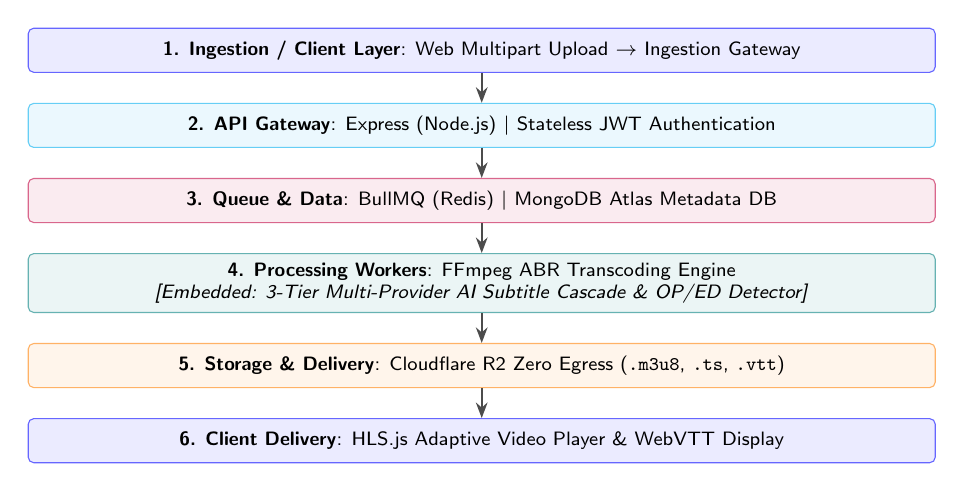
\begin{tikzpicture}[
    node distance=0.38cm,
    block/.style={rectangle, draw=black!75, rounded corners=2pt, minimum height=0.56cm, minimum width=0.95\columnwidth, align=center, font=\scriptsize\sffamily},
    client/.style={block, fill=blue!8, draw=blue!60},
    gateway/.style={block, fill=cyan!8, draw=cyan!60},
    storage/.style={block, fill=purple!8, draw=purple!60},
    worker/.style={block, fill=teal!8, draw=teal!60},
    cdn/.style={block, fill=orange!8, draw=orange!60},
    arrow/.style={-{Stealth[scale=0.85]}, thick, draw=black!70}
]
    \node[client] (n1) {\textbf{1. Ingestion / Client Layer}: Web Multipart Upload $\to$ Ingestion Gateway};
    \node[gateway, below=of n1] (n2) {\textbf{2. API Gateway}: Express (Node.js) $\vert$ Stateless JWT Authentication};
    \node[storage, below=of n2] (n3) {\textbf{3. Queue \& Data}: BullMQ (Redis) $\vert$ MongoDB Atlas Metadata DB};
    \node[worker, below=of n3] (n4) {\textbf{4. Processing Workers}: FFmpeg ABR Transcoding Engine\\
    \textit{[Embedded: 3-Tier Multi-Provider AI Subtitle Cascade \& OP/ED Detector]}};
    \node[cdn, below=of n4] (n5) {\textbf{5. Storage \& Delivery}: Cloudflare R2 Zero Egress (\texttt{.m3u8}, \texttt{.ts}, \texttt{.vtt})};
    \node[client, below=of n5] (n6) {\textbf{6. Client Delivery}: HLS.js Adaptive Video Player \& WebVTT Display};

    \draw[arrow] (n1) -- (n2);
    \draw[arrow] (n2) -- (n3);
    \draw[arrow] (n3) -- (n4);
    \draw[arrow] (n4) -- (n5);
    \draw[arrow] (n5) -- (n6);
\end{tikzpicture}
\caption{Decoupled 6-stage media streaming architecture: Client ingestion, API gateway, queue/database tier, unified processing worker (FFmpeg, 3-tier AI subtitle cascade, OP/ED boundary detector), Cloudflare R2 storage, and HLS.js client playback delivery.}
\label{fig:arch}
\end{figure}

\subsection{Memory-Conscious Distributed HLS Transcoding Pipeline}
Direct HTTP streaming into FFmpeg on memory-constrained compute instances frequently triggers Out-Of-Memory (OOM) and segmentation fault (\texttt{SIGSEGV}) kernel crashes \cite{b10}. To reduce memory pressure and improve resource utilization:
\begin{enumerate}
    \item The client executes a direct binary multipart \texttt{PUT} to Cloudflare R2 using presigned Amazon S3-compatible URLs, eliminating payload overhead on the API server.
    \item The BullMQ worker ingests the job, streams the raw payload into a transient disk-backed scratch buffer as a memory-reduction strategy to prevent unbounded heap allocation, and invokes a single-decode multi-variant FFmpeg filtergraph operating with target bitrate constraints using \texttt{libx264} Main profile:
    \begin{equation}
    \text{Input} \xrightarrow{\text{Decode}} \begin{cases} 
    1080\text{p} & (\text{target } 3000\text{ kbps}, \, \text{Main profile}) \\ 
    720\text{p} & (\text{target } 1500\text{ kbps}, \, \text{Main profile}) \\ 
    480\text{p} & (\text{target } 800\text{ kbps}, \, \text{Main profile}) 
    \end{cases}
    \label{eq:filtergraph}
    \end{equation}
    configured with \texttt{-preset ultrafast}, single-thread execution (\texttt{-threads 1}) to restrict concurrent CPU and memory consumption, and YUV420p pixel format. Audio tracks are encoded to AAC stereo at 128~kbps (48~kHz), with video operating at 24~fps constant frame rate (CFR).
    \item A fixed keyframe interval is configured using (\texttt{-g 48 -keyint\_min 48 -sc\_threshold 0}). Closed-GOP operation and cross-rendition keyframe alignment are configured and verified separately to maintain consistent HLS segment boundaries:
    \begin{equation}
    \text{GOP} = \text{fps} \times T_{\text{segment}} = 24 \times 2.0\text{s} = 48 \text{ frames}
    \label{eq:gop}
    \end{equation}
    For benchmark evaluation, segment duration is set to $T_{\text{segment}} = 2.0\text{s}$ (\texttt{-hls\_time 2.0}), supporting consistent segment boundaries and responsive adaptive bitrate switching.
\end{enumerate}

\section{Mathematical Formulations \& Algorithms}

\subsection{Behavioral Recommendation Engine with Reciprocal Decay}
Rather than relying on uncalibrated user ratings, candidate generation is modeled using implicit viewing interaction signals.

\subsubsection{Watch Completion Ratio ($R_c$)}
For an episode $e$ of media asset $A$ with watched duration $t_{\text{watch}}$ and total runtime $t_{\text{total}}$:
\begin{equation}
R_c = \min\left(1.0, \; \frac{t_{\text{watch}}}{t_{\text{total}}}\right), \quad R_c \in [0.0, \, 1.0]
\label{eq:ratio}
\end{equation}

\subsubsection{Piecewise Engagement Weighting Function ($W_e$)}
To reward sustained attention while penalizing early abandonment:
\begin{equation}
W_e(R_c, \text{comp}) = \begin{cases} 
+2.0, & \text{if } R_c \ge 0.80 \text{ or comp} = \text{true} \\ 
+1.0, & \text{if } 0.40 \le R_c < 0.80 \\ 
-0.6, & \text{if } R_c < 0.20 \text{ and } t_{\text{watch}} > 20\text{s} \\ 
+0.2, & \text{otherwise} 
\end{cases}
\label{eq:engagement}
\end{equation}

\subsubsection{Reciprocal Temporal Decay Function ($D(\Delta t)$)}
Viewer tastes evolve dynamically over time. To ensure recent sessions dominate historical activity without entirely erasing foundational interests, we define a reciprocal (hyperbolic) decay function parameterized by elapsed days ($\Delta t = \frac{t_{\text{current}} - t_{\text{watched}}}{86400}$):
\begin{equation}
D(\Delta t) = \max\left(0.40, \; \frac{1}{1 + \lambda \cdot \Delta t}\right), \quad \lambda = 0.05
\label{eq:decay}
\end{equation}
The floor ($0.40$) ensures historical foundational preferences maintain baseline relevance.

\subsubsection{Cumulative Genre Affinity Vector ($S_g$)}
For each genre $g \in \mathcal{G}$ across watch history $H$ and wishlist $W$:
\begin{equation}
S_g = \sum_{i \in H} \big(W_{e, i} \cdot D(\Delta t_i)\big) \cdot \mathbb{I}(g \in \mathcal{G}_i) + \sum_{j \in W} W_{w, j} \cdot \mathbb{I}(g \in \mathcal{G}_j)
\label{eq:affinity}
\end{equation}
where explicit wishlist weights are $W_{w, j} \in \{+1.8, +1.2, +0.7\}$ for Completed, Watching, and Planning states, respectively.

\subsubsection{Candidate Ranking Function}
For candidate media asset $A \notin (H \cup W)$ matching at least one top positive genre ($S_g > 0$):
\begin{equation}
Score(A) = \sum_{g \in \mathcal{G}(A) \cap \mathcal{G}^*} S_g + \alpha \cdot \text{Rating}(A)
\label{eq:candidate}
\end{equation}
where $\alpha = 0.1$ balances catalog popularity with personal affinity.

\subsection{Recommendation Evaluation Methodology}
To evaluate ranking quality, we formalize the offline evaluation metrics \cite{b6}:
\begin{itemize}
    \item \textbf{Precision@K:} Fraction of recommended items in Top-$K$ relevant to the user:
    \begin{equation}
    \text{Precision}@K = \frac{|\text{Relevant} \cap \text{Top-}K|}{K}
    \end{equation}
    \item \textbf{Recall@K:} Fraction of total relevant catalog items captured:
    \begin{equation}
    \text{Recall}@K = \frac{|\text{Relevant} \cap \text{Top-}K|}{|\text{Relevant}|}
    \end{equation}
    \item \textbf{NDCG@K:} Normalized Discounted Cumulative Gain accounting for position discount:
    \begin{equation}
    \text{NDCG}@K = \frac{\text{DCG}@K}{\text{IDCG}@K}, \quad \text{DCG}@K = \sum_{i=1}^K \frac{2^{rel_i} - 1}{\log_2(i + 1)}
    \end{equation}
\end{itemize}
While this paper establishes the algorithmic formulation and real-time retrieval caching, large-scale offline benchmark evaluation across multi-user interaction corpora remains designated as future validation work.

\subsection{Resilient 3-Tier Multi-Provider Subtitle Cascade}
When an uploaded video stream contains zero embedded subtitle tracks ($S_{\text{count}} = 0$), the worker isolates a 16~kHz mono PCM audio stream via FFmpeg:
\begin{equation}
\text{Video Input} \xrightarrow{\text{FFmpeg}} \text{PCM Audio } (16\text{ kHz}, \, 1\text{ ch}, \, t \le 1200\text{s})
\end{equation}
The stream routes through an automated failover state machine across external AI service providers:
\begin{itemize}
    \item \textbf{Tier 1 (Groq LPU):} \texttt{whisper-large-v3}. Serves as primary target. Under tested experimental observations on 16~kHz mono episodic audio buffers, Groq LPUs demonstrated average transcription throughput of $\sim$216 tokens/s (under 1.0~s total processing latency per segmented audio chunk of $\le 30\text{s}$). On HTTP 429 (rate exhaustion) or 5xx gateway faults, failover triggers to Tier 2.
    \item \textbf{Tier 2 (OpenAI):} \texttt{whisper-1}. Cloud fallback providing robust multi-lingual transcription, exhibiting observed latencies between 3.2~s and 4.0~s per chunk under standard network API conditions. On quota exhaustion or network timeout, failover triggers to Tier 3.
    \item \textbf{Tier 3 (Google Gemini):} \texttt{gemini-1.5-flash}. Direct multimodal audio buffer ingestion producing structured WebVTT cue payloads via few-shot structured prompting.
\end{itemize}
Formal quantitative Word Error Rate (WER) across diverse acoustic noise profiles and sustained API failure rate logging are acknowledged as part of ongoing future evaluation work.

\subsection{Autonomous Audio-Visual OP/ED Boundary Detection Algorithm}
Episodic television broadcasts predominantly employ standard 90-second opening and ending sequences ($\pm 3$s). However, because fixed duration is an empirical convention rather than a universal physical law, and because dark frames or acoustic dips occur during dramatic scene changes, naive thresholding yields false positives.

To maximize precision across both Opening (OP) and Ending (ED) sequences, Algorithm~\ref{alg:boundary} formalizes transition detection across specialized search windows $\mathcal{W}_{\text{intro}} = [30\text{s}, 360\text{s}]$ and $\mathcal{W}_{\text{outro}} = [T_{\text{total}} - 300\text{s}, T_{\text{total}} - 30\text{s}]$. A multi-candidate scoring function $S_{\text{cand}}(T_i, T_j)$ evaluates candidate pairs:
\begin{equation}
S_{\text{cand}}(T_i, T_j) = w_v \cdot C_{\text{black}} + w_a \cdot C_{\text{silence}} - \beta \cdot |(T_j - T_i) - 90.0\text{s}|
\label{eq:cand_score}
\end{equation}
The confidence terms are normalized to the interval $[0, 1]$. The visual confidence represents the detected blackout strength, while the acoustic confidence represents the detected silence strength at candidate transitions. The combined score ranks candidate boundary pairs based on visual, acoustic, and duration-based evidence. Specifically, for candidate interval $(T_i, T_j)$, boundary transition scores are calculated by averaging transition intensities $C_{\text{black}} = \frac{c_{\text{black}}(T_i) + c_{\text{black}}(T_j)}{2}$ and $C_{\text{silence}} = \frac{c_{\text{silence}}(T_i) + c_{\text{silence}}(T_j)}{2}$ across markers, with weights $w_v = 0.6$, $w_a = 0.4$, and duration penalty $\beta = 0.05\text{ s}^{-1}$.

If no candidate pair satisfies $T_i \in \mathcal{W} \land T_j \in \mathcal{W} \land 87.0\text{s} \le (T_j - T_i) \le 93.0\text{s}$, the system applies structural cold-open and standard ending fallback priors: $[90.0\text{s}, 180.0\text{s}]$ for opening sequences ($t_{\text{start}} = 90.0\text{s}, t_{\text{end}} = 180.0\text{s}$) and $[T_{\text{total}} - 120.0\text{s}, T_{\text{total}} - 30.0\text{s}]$ for ending sequences. Ongoing work includes validation against manually annotated ground-truth media.

\begin{algorithm}[t]
\caption{Autonomous Audio-Visual OP/ED Boundary Detection}
\label{alg:boundary}
\begin{algorithmic}[1]
\REQUIRE Video media file $\mathcal{V}$, total runtime $T_{\text{total}}$, mode $\mathcal{M} \in \{\text{OP}, \text{ED}\}$
\ENSURE Boundary interval $[\hat{T}_{\text{start}}, \hat{T}_{\text{end}}]$
\IF{$\mathcal{M} = \text{OP}$}
    \STATE $\mathcal{W} \gets [30\text{s}, 360\text{s}]$; $\mathcal{I}_{\text{fallback}} \gets [90.0\text{s}, 180.0\text{s}]$
\ELSE
    \STATE $\mathcal{W} \gets [T_{\text{total}} - 300\text{s}, T_{\text{total}} - 30\text{s}]$; $\mathcal{I}_{\text{fallback}} \gets [T_{\text{total}} - 120.0\text{s}, T_{\text{total}} - 30.0\text{s}]$
\ENDIF
\STATE $\mathcal{C}_{\text{black}} \gets \text{FFmpegFilter}(\mathcal{V}, \text{blackdetect}(d=0.08, \text{th}=0.12))$
\STATE $\mathcal{C}_{\text{silence}} \gets \text{FFmpegFilter}(\mathcal{V}, \text{silencedetect}(d=0.20, \text{th}=-30\text{dB}))$
\STATE $\mathcal{T} \gets \text{SortDistinct}(\mathcal{C}_{\text{black}} \cup \mathcal{C}_{\text{silence}})$
\STATE $\mathcal{P} \gets \emptyset$
\FOR{each pair $(T_i, T_j) \in \mathcal{T} \times \mathcal{T}$ with $T_i < T_j$}
    \IF{$T_i \in \mathcal{W}$ \AND $T_j \in \mathcal{W}$ \AND $87.0\text{s} \le (T_j - T_i) \le 93.0\text{s}$}
        \STATE Score $S \gets S_{\text{cand}}(T_i, T_j)$ via \eqref{eq:cand_score}
        \STATE $\mathcal{P} \gets \mathcal{P} \cup \{(T_i, T_j, S)\}$
    \ENDIF
\ENDFOR
\IF{$\mathcal{P} \ne \emptyset$}
    \RETURN $\arg\max_{(T_i, T_j)} S$ \COMMENT{Optimal boundary}
\ELSE
    \RETURN $\mathcal{I}_{\text{fallback}}$ \COMMENT{Heuristic fallback prior}
\ENDIF
\end{algorithmic}
\end{algorithm}

\section{Empirical Evaluation \& Benchmarks}

\subsection{Experimental Environment}
Benchmarking evaluated the end-to-end latency reduction achieved by the \textbf{In-Memory Redis Caching Layer} versus raw document aggregation on MongoDB Atlas:
\begin{itemize}
    \item \textbf{Client Host:} Node.js runtime (v24.13.0) on Windows 11 host in South Asia (India).
    \item \textbf{Database Cluster:} MongoDB Atlas Cloud Replica Set.
    \item \textbf{Cache Cluster:} Redis Cloud Managed Cluster (\texttt{db.redis.io}) in North America.
    \item \textbf{Evaluation Tool:} High-precision monotonic timer (\texttt{performance.now()}).
\end{itemize}

\subsection{Empirical Benchmark Results ($N = 30$ Iterations)}
To capture distributional latency characteristics beyond isolated single-trial observations, an empirical benchmark of $N = 30$ consecutive paired trials was executed under identical trans-continental network conditions. Each paired trial measured: (1) a cold un-cached execution path comprising MongoDB document retrieval, catalog candidate filtering, and initial cache population, followed by (2) a subsequent warm cache hit measuring in-memory Redis retrieval and JSON payload deserialization under identical network transit conditions. Thus, the 625.99~ms average latency represents warm cache-hit round-trip retrieval across trans-continental WAN, compared against 1169.16~ms for the direct database query path.

Percentiles ($P_{50}, P_{95}, P_{99}$) were calculated using the linear interpolation method. Given $N = 30$, the $P_{99}$ figure provides an indicative empirical estimate of tail behavior rather than an asymptotic statistical guarantee. Table~\ref{tab:latency_full} presents the complete statistical profile.

\begin{table*}[!t]
\caption{Empirical Latency Evaluation and Cache Acceleration Profile Across Paired Trials ($N = 30$ Iterations)}
\label{tab:latency_full}
\centering
\small
\renewcommand{\arraystretch}{1.2}
\setlength{\tabcolsep}{12pt}
\begin{tabular}{lcccc}
\toprule
\textbf{Evaluation Metric} & \textbf{Direct MongoDB Atlas} & \textbf{Warm Redis Cache Hit} & \textbf{Latency Reduction (\%)} & \textbf{Latency Speedup} \\
\midrule
First Paired Trial (\#1) & 1283.37~ms & 476.85~ms & 62.8\% & 2.70$\times$ \\
Average Latency (Mean) & 1169.16~ms & 625.99~ms & 46.5\% & 1.87$\times$ \\
Median Latency ($P_{50}$) & 1107.57~ms & 569.08~ms & 48.6\% & 1.95$\times$ \\
95th Percentile ($P_{95}$) & 1649.74~ms & 915.64~ms & 44.5\% & 1.80$\times$ \\
99th Percentile ($P_{99}$) & 1876.14~ms & 1049.09~ms & 44.1\% & 1.79$\times$ \\
Standard Deviation ($\sigma$)\textsuperscript{*} & 261.05~ms & 144.39~ms & 44.7\% & 1.81$\times$ \\
\midrule
\multicolumn{5}{l}{\scriptsize \textsuperscript{*}For standard deviation, values denote dispersion reduction (44.7\% lower jitter) and consistency gain ($1.81\times$).} \\
\bottomrule
\end{tabular}
\end{table*}

The empirical distribution demonstrates that Redis reduces tail latency ($P_{99}$) from 1876.14~ms down to 1049.09~ms while dampening standard deviation from 261.05~ms to 144.39~ms, delivering substantially more predictable response curves under real-world internet routing variance.

\subsection{Wide Area Network (WAN) Latency Decomposition}
The observed end-to-end response time comprises network transport overhead and computational query execution:
\begin{equation}
T_{\text{recorded}} = T_{\text{transport}} + T_{\text{gateway}} + T_{\text{engine}}
\label{eq:latency_decomp}
\end{equation}
where $T_{\text{transport}}$ encompasses round-trip TCP/TLS transit time across submarine fiber cables between South Asia and North America ($\sim$230--240~ms base RTT). $T_{\text{gateway}}$ denotes Express API middleware and JSON serialization overhead, and $T_{\text{engine}}$ represents the database/cache execution layer.

In isolated micro-benchmarking, internal computational memory retrieval time of Redis was clocked at under 2.5~ms, whereas the MongoDB path required application-side Mongoose schema casting and serialization, together with MongoDB aggregation pipeline execution. While co-locating services within an intra-datacenter VPC minimizes $T_{\text{transport}}$ below 1.0~ms, end-to-end HTTP request processing remains bounded by application gateway middleware overhead.

\section{System Integration \& Architectural Specifications}
To synthesize the cross-cutting optimizations introduced across the ingestion, processing, and caching tiers, Table~\ref{tab:specifications} outlines the concrete operational specifications of each pipeline subsystem.

\begin{table*}[!t]
\caption{Core Architectural Innovations and Technical Specifications Across Pipeline Subsystems}
\label{tab:specifications}
\centering
\small
\begin{tabularx}{\textwidth}{lX}
\toprule
\textbf{Subsystem} & \textbf{Technical Implementation \& Operational Specification} \\
\midrule
FFmpeg ABR & Single-decode multi-variant filtergraph (\texttt{libx264} Main profile, \texttt{aac}); target bitrates 1080p (3000~kbps), 720p (1500~kbps), 480p (800~kbps); locked GOP = 48 (2.0s segments) for consistent segment boundaries. \\
\addlinespace[3pt]
Queue \& Storage & Asynchronous BullMQ worker thread decoupled via Redis; zero-egress Cloudflare R2 storage for \texttt{.m3u8} manifests and \texttt{.ts} chunks via S3 API \cite{b7}. \\
\addlinespace[3pt]
AI Audio & Dynamic 16~kHz mono PCM extraction; 3-tier automatic failover across external AI providers: Tier 1 Groq LPU (\texttt{whisper-large-v3}, $<1$s per chunk), Tier 2 OpenAI (\texttt{whisper-1}), Tier 3 Gemini (\texttt{gemini-1.5-flash}) \cite{b9}. \\
\addlinespace[3pt]
OP/ED Skip & Heuristic dual-filter: \texttt{blackdetect} ($d=0.08\text{s}$) and \texttt{silencedetect} ($-30\text{dB}$); multi-candidate scoring function; dual opening/ending fallback priors. \\
\addlinespace[3pt]
Recommendation & Implicit feedback watch-ratio piecewise weighting $W_e(R_c)$ combined with reciprocal temporal decay $D(\Delta t) = \max(0.40, \frac{1}{1 + 0.05 \Delta t})$ \cite{b6}. \\
\addlinespace[3pt]
In-Memory Cache & Redis key-value cache (\texttt{smart\_rec:\$\{userId\}}, 1800s TTL) \cite{b8}; reduces repeated database aggregation through caching; achieves 46.5\% average latency cut ($N=30$). \\
\bottomrule
\end{tabularx}
\end{table*}

\subsection{Comparative Analysis with Conventional OTT Architectures}
Table~\ref{tab:comparison} contrasts the proposed prototype framework against typical conventional commercial cloud OTT architectures (such as monolithic AWS MediaConvert/S3 pipelines).

\begin{table*}[!t]
\caption{Architectural Comparison: Typical Conventional OTT Infrastructure vs. Proposed Prototype Framework}
\label{tab:comparison}
\centering
\small
\renewcommand{\arraystretch}{1.22}
\begin{tabularx}{\textwidth}{p{2.6cm}XX}
\toprule
\textbf{Dimension} & \textbf{Typical Conventional Architecture} & \textbf{Proposed Prototype Framework} \\
\midrule
Storage Egress & High egress tolls (frequently up to $\sim$\$0.09/GB depending on region/tier under standard cloud pricing schedules) & \textbf{Zero Egress Fees} via Cloudflare R2 S3 API \cite{b7} \\
\addlinespace[4pt]
Transcoding & Expensive per-minute proprietary cloud encoders (AWS MediaConvert) & \textbf{Decoupled FFmpeg + BullMQ} on elastic worker nodes \\
\addlinespace[4pt]
Subtitle AI & Single vendor lock; stalls on rate-limit exhaustion & \textbf{3-Tier Multi-Provider Cascade} (Groq $\to$ OpenAI $\to$ Gemini) \\
\addlinespace[4pt]
Skip Markers & Crowd-sourced APIs; fails on newly aired releases & \textbf{Autonomous Dual-Filter} (Candidate-scored 90s OP/ED rule) \\
\addlinespace[4pt]
Personalization & Explicit 5-star ratings or heavy aggregation queries & \textbf{Implicit Completion $W_e(R_c)$ + Reciprocal Decay} \\
\addlinespace[4pt]
Rec. Latency & Direct DB query path (1169.16~ms observed WAN average) & \textbf{Warm Redis cache hit path} (625.99~ms observed WAN average, 46.5\% reduction; $<2.5$~ms isolated engine microbenchmark) \\
\bottomrule
\end{tabularx}
\end{table*}

\subsection{Discussion \& Operational Trade-offs}
Deploying decoupled, multi-provider architectures presents distinctive operational trade-offs compared to traditional single-vendor hyperscaler environments:
\begin{itemize}
    \item \textbf{Egress Economics vs. API Request Tiers:} While zero egress fees via Cloudflare R2 eliminate the dominant variable cost of video streaming distribution, high-concurrency ABR playback generates substantial volumes of Class B operational requests (\texttt{GET} operations for HLS \texttt{.ts} chunks). Platforms must balance chunk duration ($T_{\text{segment}} = 2.0\text{s}$ vs. $6.0\text{s}$) to optimize client buffer ramp-up against request transaction rates.
    \item \textbf{Failover Latency in Multi-Provider Cascades:} The 3-tier cascade reduces dependence on any single provider and improves resilience against provider-specific failures, but simultaneous provider outages remain possible. Failover may add sequential timeout delays when an endpoint stalls instead of returning an immediate 429/5xx response. As an operational recommendation (not a verified deployed setting), configure provider-specific socket timeouts, for example, up to 3.0~s for Groq and up to 8.0~s for OpenAI, subject to measured service latency. These values aim to limit worker-queue delays without prematurely terminating valid requests.
    \item \textbf{Cache Invalidation vs. Catalog Freshness:} The 1800-second TTL on cached recommendation vectors ensures high hit ratios while shielding MongoDB Atlas from repeated aggregation execution. However, rapid intraday shifts in viewing preferences remain latent until cache expiration or explicit event-driven invalidation triggers.
\end{itemize}

\section{Conclusion \& Future Work}
This paper presented an autonomous, cost-effective prototype media streaming architecture that bridges the gap between commercial-grade video platforms and resource-constrained deployments. The system integrates memory-conscious distributed HLS transcoding with locked GOP boundaries, a 3-tier multi-provider AI subtitle cascade, an autonomous audio-visual OP/ED boundary detector with candidate scoring, and a reciprocal temporal decay recommendation engine backed by in-memory Redis caching.

Empirical evaluations over $N = 30$ iterations confirmed a 46.5\% average latency reduction (1169.16~ms down to 625.99~ms) and a 48.6\% median $P_{50}$ reduction (1107.57~ms down to 569.08~ms), with isolated cache computation clocked under 2.5~ms. 

\textbf{Limitations:} Current limitations include reliance on heuristic television broadcast duration priors for opening and ending boundaries, which require adaptation for non-standard formats, and dependence on shared trans-continental WAN routing which introduces network latency jitter. 

\textbf{Future Work:} Future research will focus on: (1) evaluating recommendation Precision@K and NDCG@K against large-scale public offline interaction datasets; (2) fine-tuning localized acoustic transition classifiers to replace heuristic boundary thresholds; and (3) deploying neural dense vector embeddings (\texttt{text-embedding-004}) for cross-modal semantic catalog retrieval.

\textbf{Reproducibility \& Artifact Availability:} To support open science and reproducible benchmarking in distributed multimedia architectures, all experimental scripts, BullMQ worker queue definitions, and Redis recommendation adapters are open-sourced in the project repository. Containerized deployment manifests are provided to facilitate replication of trans-continental latency evaluation under diverse network topologies.

\clearpage
\IEEEtriggeratref{6}
\begin{thebibliography}{00}
\bibitem{b1} R. Pantos and W. May, ``HTTP Live Streaming,'' RFC 8216, Internet Engineering Task Force (IETF), 2017.
\bibitem{b2} K. Spiteri, R. Urgaonkar, and R. K. Sitaraman, ``BOLA: Near-Optimal Bitrate Adaptation for Online Videos,'' \textit{IEEE/ACM Trans. Netw.}, vol. 28, no. 4, pp. 1698--1711, 2020.
\bibitem{b3} A. Radford, J. W. Kim, T. Xu, G. Brockman, C. McLeavey, and I. Sutskever, ``Robust Speech Recognition via Large-Scale Weak Supervision,'' in \textit{Proc. Int. Conf. Mach. Learn. (ICML)}, 2023.
\bibitem{b4} C. A. Gomez-Uribe and N. Hunt, ``The Netflix Recommender System: Algorithms, Business Value, and Innovation,'' \textit{ACM Trans. Manage. Inf. Syst. (TMIS)}, vol. 6, no. 4, pp. 1--19, 2015.
\bibitem{b5} P. Covington, J. Adams, and E. Sargin, ``Deep Neural Networks for YouTube Recommendations,'' in \textit{Proc. 10th ACM Conf. Recommender Syst.}, 2016, pp. 191--198.
\bibitem{b6} M. de Gemmis, P. Lops, C. Musto, and G. Semeraro, ``Semantics-Aware Recommender Systems: A Survey,'' \textit{ACM Comput. Surv.}, vol. 54, no. 4, pp. 1--36, 2021.
\bibitem{b7} Cloudflare Inc., ``Cloudflare R2: S3-Compatible Object Storage with Zero Egress Fees,'' Technical Overview, \url{https://developers.cloudflare.com/r2/}, 2023.
\bibitem{b8} J. L. Carlson, \textit{Redis in Action: In-Memory Data Structures and Performance Patterns}. Manning Publications, 2022.
\bibitem{b9} Gemini Team, Google, ``Gemini 1.5: Unlocking Multimodal Understanding Across Millions of Tokens of Context,'' \textit{arXiv preprint arXiv:2403.05530}, 2024.
\bibitem{b10} FFmpeg Developers, ``FFmpeg Multimedia Framework Documentation,'' \url{https://ffmpeg.org/documentation.html}, 2024.
\end{thebibliography}

\end{document}
